\documentclass[tikz,border=5pt]{standalone}
\usepackage{pgfplots}
\pgfplotsset{compat=1.18}

\definecolor{corba}{HTML}{365FB3}
\definecolor{punt}{HTML}{B91C1C}
\definecolor{guia}{HTML}{6B7280}

\begin{document}
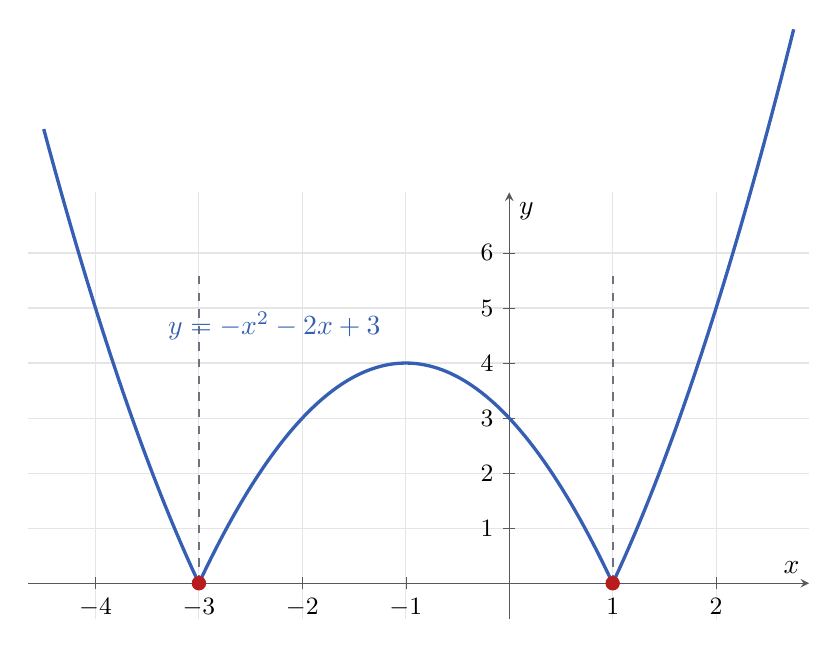
\begin{tikzpicture}
  \begin{axis}[
    width=11.5cm,
    height=7cm,
    axis lines=middle,
    xmin=-4.65,
    xmax=2.9,
    ymin=-0.65,
    ymax=7.1,
    xlabel={$x$},
    ylabel={$y$},
    xtick={-4,-3,-2,-1,0,1,2},
    ytick={1,2,3,4,5,6},
    grid=major,
    grid style={black!10},
    axis line style={black!65},
    tick style={black!65},
    tick label style={font=\small},
    clip=false,
  ]
    \addplot[corba, very thick, domain=-4.5:-3, samples=100]
      {x^2+2*x-3};
    \addplot[corba, very thick, domain=-3:1, samples=130]
      {-x^2-2*x+3};
    \addplot[corba, very thick, domain=1:2.75, samples=100]
      {x^2+2*x-3};
    \addplot[only marks, mark=*, mark size=2.4pt, punt]
      coordinates {(-3,0) (1,0)};
    \draw[guia, dashed, thick]
      (axis cs:-3,0) -- (axis cs:-3,5.6);
    \draw[guia, dashed, thick]
      (axis cs:1,0) -- (axis cs:1,5.6);
    \node[anchor=south east, text=corba] at (axis cs:-1.15,4.25)
      {$y=-x^2-2x+3$};
  \end{axis}
\end{tikzpicture}
\end{document}
